\chapter{Resultados}
\label{chap:resultados}
\section{Análise exploratória dos dados do POLYMOD}

A partir da coleta de dados realizada pelo POLYMOD, o propósito é elucidar a estruturação das interconexões interpessoais e analisar as implicações decorrentes dessas relações visando uma modelagem em redes. Para isso cada indivíduo foi categorizado em 5 faixas etárias: [0,20) (jovens), [20,30) (jovens adultos), [30,50) (adultos), [50,70) (adultos \textit{seniors}) e maiores de 70 que representam os idosos; a distribuição de cada faixa etária é mostrada na Figura \ref{fig:freq} que foi obtida a partir do Censo de 2022 do IBGE \cite{ibgeCenso2022}. Esta categorização reveste-se de relevância considerável, haja vista que a estimação dos parâmetros utilizados é viável com a categorização das idades e será distribuição de idades na red.

\begin{figure}[H]
    \centering

    \captionsetup{font=normalsize,skip=0.8pt,singlelinecheck=on,labelsep=endash}
    \caption{Faixas etárias do Brasil}
    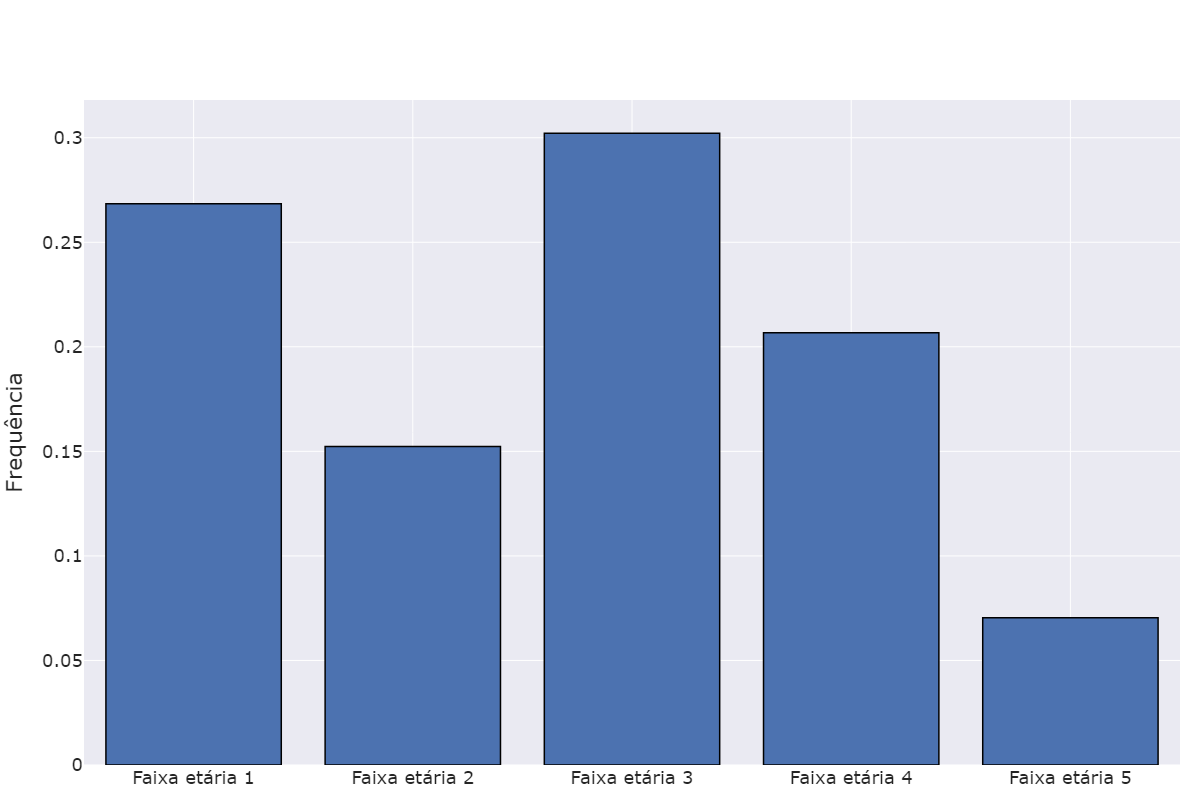
\includegraphics[scale= 0.4]{figuras/faixas_brasil.png}
    \captionsetup{font=small,justification=justified}
    \caption*{Resultados da frequência de cada faixa etária no banco de dados do Censo 2022 IBGE, esse será um dos \textit{inputs} do modelo posteriormente.\\ Fonte: Autor.}

    \label{fig:freq}
\end{figure}

Com base nos dados obtidos, 
foi
realizada uma investigação para avaliar a duração, frequência e a presença de contato físico nos encontros em análise. A Figura \ref{fig:graficos} mostra os padrões dos contatos do POLYMOD; é possível ver que quanto mais frequente ou  
longo
é o contato maior a chance dele ter contato físico.
Além disso, quanto mais frequente é o contato maiores as chances da conversa durar mais, por exemplo em contatos diários existe mais de 50\% de chance de que o contato dure mais que 1 hora. Por fim, 
o último gráfico da Figura \ref{fig:graficos}
evidencia que, no ambiente domiciliar, a probabilidade de ocorrência de contato físico é significativamente maior.
Por contraste, no ambiente profissional, as chances são substancialmente menores, sendo considerado o cenário menos propenso a esse tipo de interação.

\begin{figure}[H]
    \centering
    \captionsetup{font=normalsize,skip=0.8pt,singlelinecheck=on,labelsep=endash}
    \caption{Probabilidade de contato físico}
    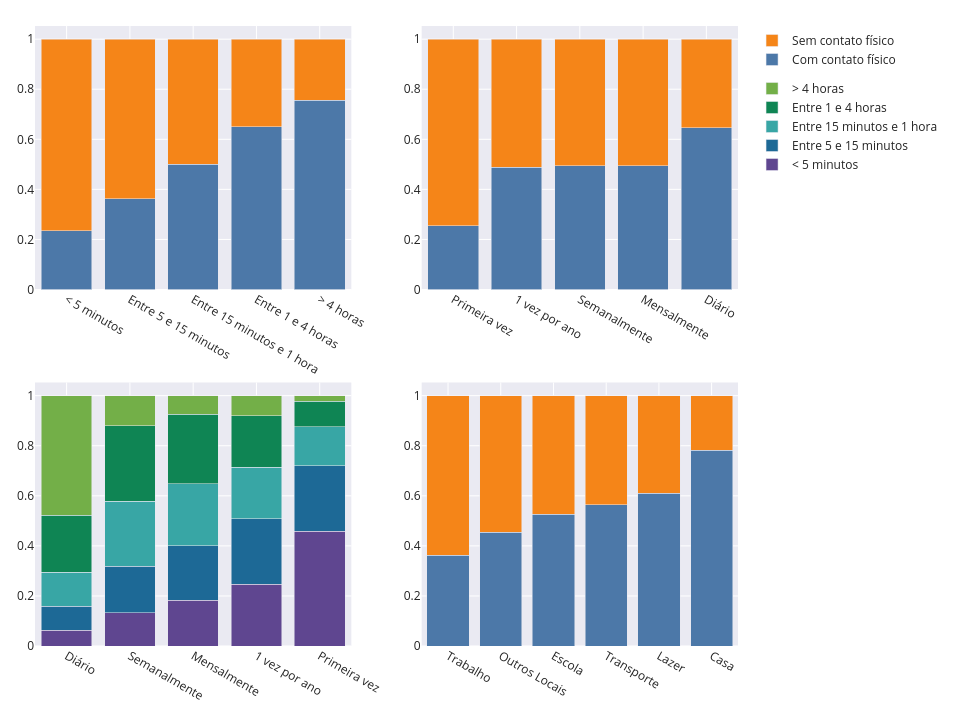
\includegraphics[scale= 0.45]{figuras/graficos-PIF.png}
\captionsetup{font=small,justification=justified}
    \caption*{Ilustra a relação entre a frequência e a duração dos contatos com a probabilidade de contato físico, mostrando que contatos mais frequentes e duradouros têm maior probabilidade de envolver contato físico. Além disso, o ambiente domiciliar apresenta maior probabilidade de contato físico, especialmente nas áreas de lazer, em comparação ao ambiente profissional, onde a probabilidade é consideravelmente menor.\\ Fonte: Autor.}
    \label{fig:graficos}
\end{figure}

Um elemento importante que foi investigado
é como as idades influenciam nas conexões entre os indivíduos da rede. A Figura \ref{fig:contatos_faixa} ilustra a distribuição de graus por faixa etária dos respondentes da pesquisa do POLYMOD.
Ao analisar a distribuição de ligações por faixa etária é percebido que a cauda segue uma distribuição geométrica, que pode ser escrita como $P \propto (1 - p)^xp$ ou $P \propto e^{-\lambda x}(1 - e^\lambda)$. 
Considerando a forma $P \propto e^{-\lambda x}(1 - e^\lambda)$, na Figura \ref{fig:contatos_faixa}, determina-se o coeficiente angular $-\lambda$ e seu respectivo $R^2$, por faixa etária, através do método dos mínimos quadrados.

\begin{figure}[H]
    \centering
    \captionsetup{font=normalsize,skip=0.8pt,singlelinecheck=on,labelsep=endash}
    \caption{Influência das idades nas conexões}
    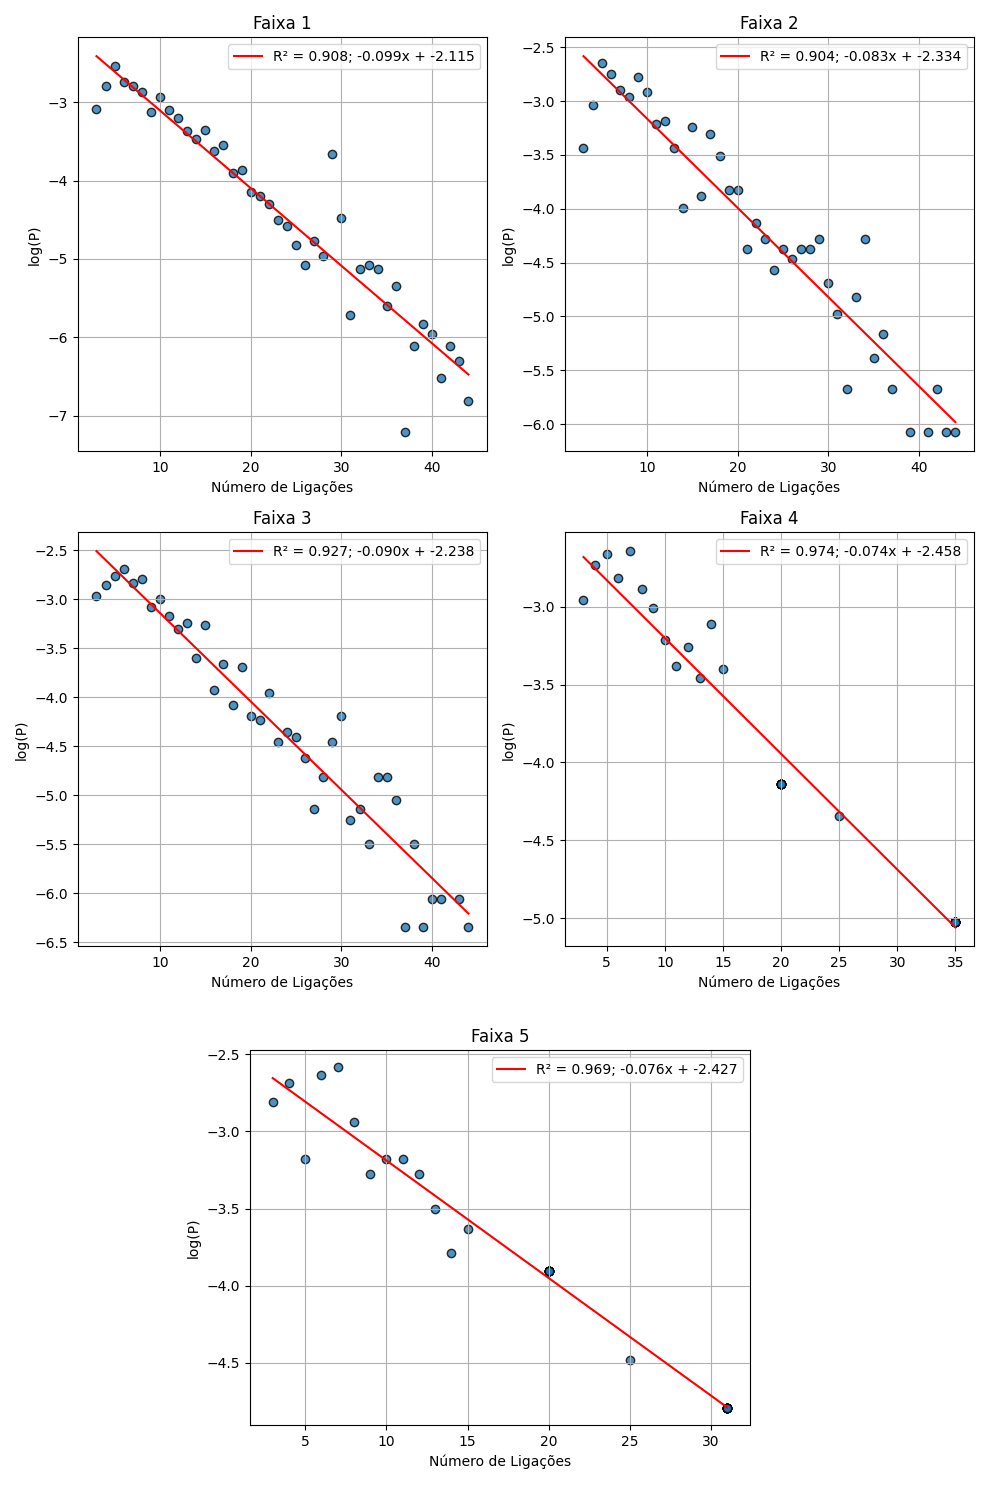
\includegraphics[scale= 0.3]{figuras/contatos_faixa.png}
    \captionsetup{font=small,justification=justified}
    \caption*{Ilustra a influência das idades nas 
    conexões da rede social, observando uma distribuição geométrica nas ligações por faixa etária.\\ Fonte: Autor.}
    \label{fig:contatos_faixa}
\end{figure}

Também foi analisada a relação entre a faixa etária de um indivíduo que preencheu o questionário do POLYMOD e a distribuição de suas ligações 
por faixas etárias.
A Figura \ref{fig:heat} ilustra para cada faixa etária das linhas, a frequência relativa de conexões com as faixas etárias das colunas. 
Independente de qual a faixa etária do indivíduo que preencheu o questionário, a maior frequência relativa de conexões é com a faixa etária 3. A faixa etária 3 é
composta majoritariamente por indivíduos que estão na fase produtiva da vida.
Em contraste, 
a menor frequência relativa de conexões se dá com a última faixa etária, devido a baixa frequência de pessoas na faixa etária.

\begin{figure}[H]
    \centering
    \captionsetup{font=normalsize,skip=0.8pt,singlelinecheck=on,labelsep=endash}
    \caption{Frequência média de conexões por faixa etária}
    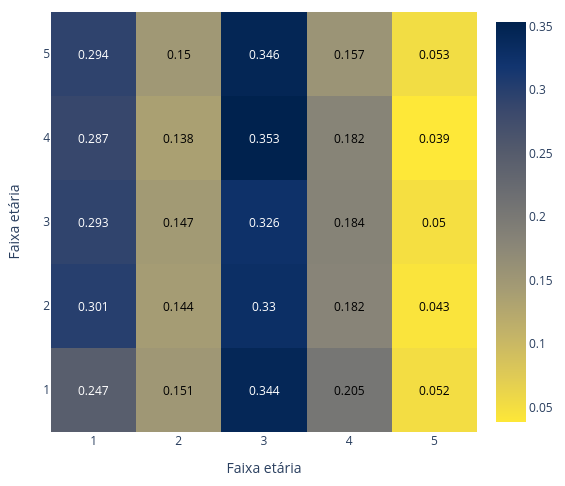
\includegraphics[scale= 0.5]{figuras/h-PIF.png}
    \captionsetup{font=small,justification=justified}
    \caption*{Mostra a frequência média de conexões por faixa etária, ressaltando que a faixa etária 3, associada à vida profissional e familiar, possui a maior frequência de conexões, enquanto a última faixa apresenta a menor frequência devido às dificuldades inerentes a essa fase da vida. \\Fonte: Autor}
    \label{fig:heat}
\end{figure}

Por último, a Figura \ref{fig:mediastd} apresenta duas matrizes de calor que ilustram a média e o desvio padrão do tempo de contato entre diferentes faixas etárias. 
Com exceção da última faixa etária, todas as outras possuem maior tempo de conexão com a faixa etária inicial. O maior tempo de conexão médio observado é entre a faixa etária 1 com ela mesma, seguida das conexões entre as faixas 1 e 3. A última faixa etária também apresenta maior tempo de conexão com ela mesma. Por outro lado, o menor tempo de conexão observado, foi entre as faixas etárias 2 e 5.


\begin{figure}[H]
    \centering
    \captionsetup{font=normalsize,skip=0.8pt,singlelinecheck=on,labelsep=endash}
    \caption{Média e desvio-padrão dos tempos de contato entre faixas etárias}
    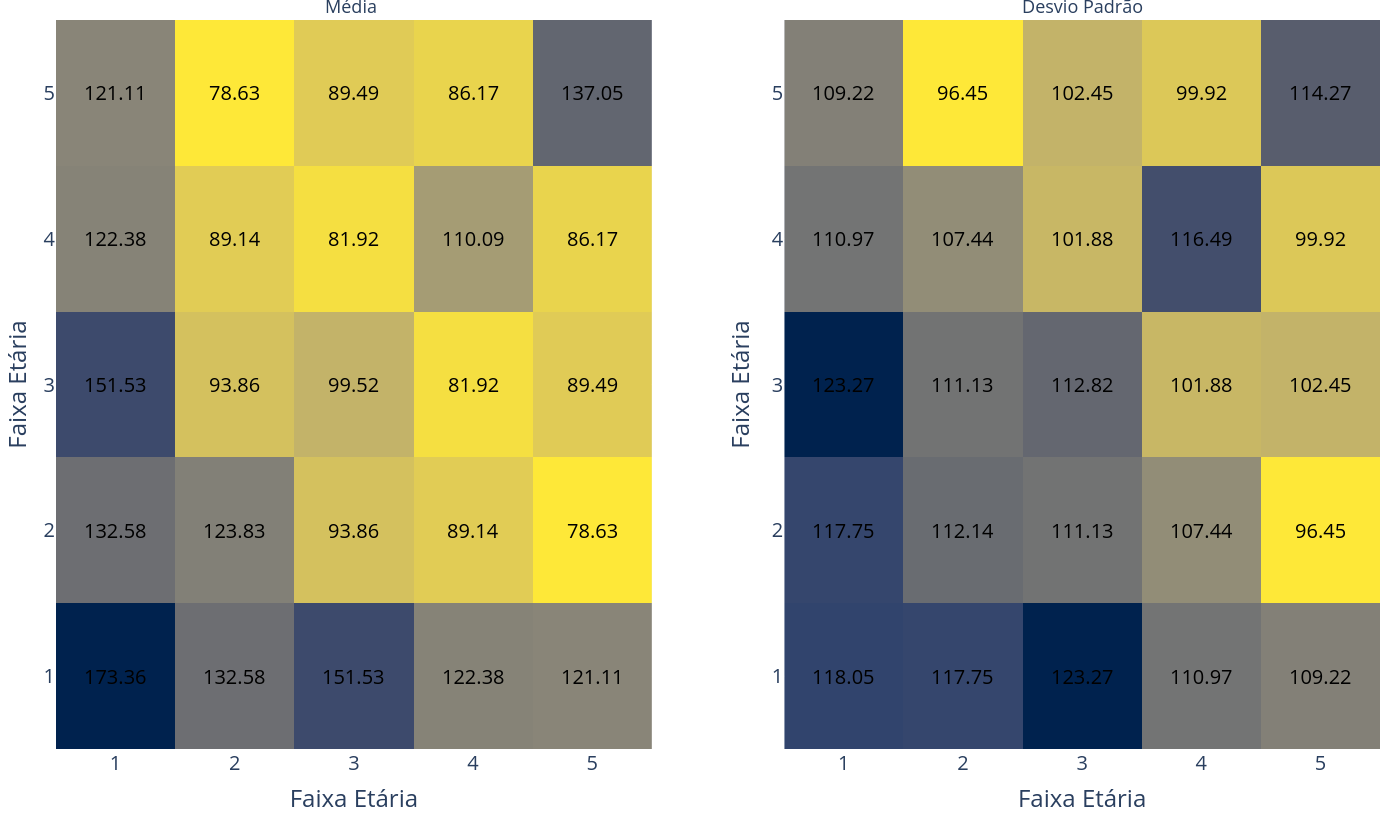
\includegraphics[scale= 0.32]{figuras/media_std.png}
    \captionsetup{font=small,justification=justified}
    \caption*{A imagem mostra a média e o desvio padrão do tempo de contato entre diferentes faixas etárias. A matriz da média indica que o contato é mais intenso dentro da mesma faixa etária e entre faixas etárias adjacentes, reduzindo conforme aumenta a diferença de idade. A matriz do desvio padrão mostra maior variação nos contatos dentro da mesma faixa e entre adjacentes, com menor variação entre faixas mais distantes. \\Fonte: Autor}
    \label{fig:mediastd}
\end{figure}
A matriz do desvio padrão indica que a variação no tempo de contato é mais significativa entre as conexões das faixas etárias 1 com as faixas etárias 1, 2 e 3. Em seguida, as maiores variabilidades observadas foram entre as faixas etárias 4 e 5 consigo mesmas. Por outro lado, a menor variabilidade foi entre as faixas etárias 2 e 5.

\section{Resultados da Rede gerada}

Os dados das Figuras \ref{fig:contatos_faixa} e \ref{fig:heat} foram utilizados como \textit{inputs} do Modelo de Configuração Ponderado \ref{alg:MCP}. Especificamente, com os dados da Figura~\ref{fig:contatos_faixa} foi obtida a distribuição empírica do grau de cada nó de cada faixa etária e com os dados da Figura~\ref{fig:heat} foram estimados os parâmetros de uma distribuição multinomial para estabelecer quantas ligações vão para cada faixa etária. A partir disso e dado um valor de $p$ (parâmetro que aumenta o coeficiente de agrupamento) foi construída a rede para acontecer a simulação da epidemia. 
A Figura \ref{fig:regressao} mostra a variação do
agrupamento com o incremento de $p$. Observa-se que o agrupamento, $C$, cresce de acordo com $C \propto p^{\alpha}$, tanto o agrupamento médio quanto o total no qual $\alpha_{medio } = 0.46$ e $\alpha_{total } = 0.55$, respectivamente. 

\begin{figure}[H]
    \centering
    \captionsetup{font=normalsize,skip=0.8pt,singlelinecheck=on,labelsep=endash}
    \caption{Agrupamento da rede em função de $p$}
    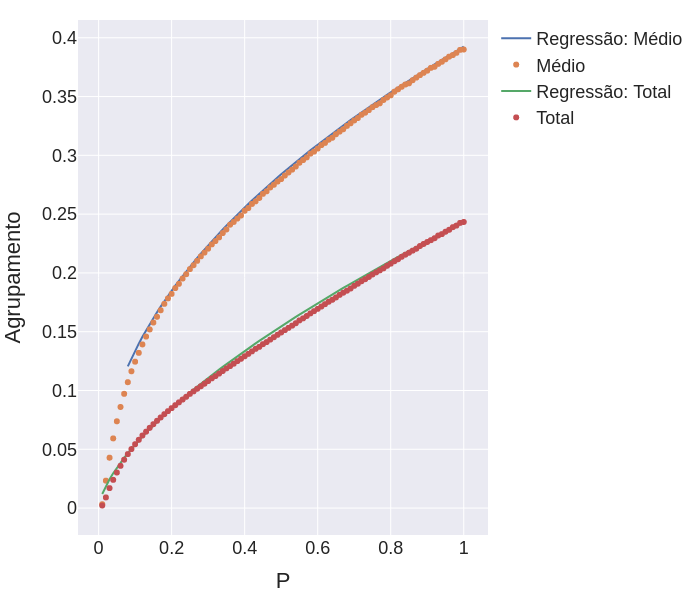
\includegraphics[scale= 0.45]{figuras/clustering_vs_p.png}
    \captionsetup{font=small,justification=justified}    \caption*{Evolução do agrupamento da rede em função 
    do incremento do valor de $p$, foi utilizada uma regressão linear para saber qual a função que rege encontrando $C \propto p^{\alpha}$ com $R^2 = 99$\%.\\Fonte: Autor}
    \label{fig:regressao}
\end{figure}

Após a 
geração da rede com o algoritmo proposto, foram calculados alguns
os dados da rede e observou-se que para qualquer valor de $p$ a distribuição de graus tinha a mesma distribuição que a encontrada pela Figura \ref{fig:contatos_faixa} a partir do teste da comparação entre modelo e dados como mostra a Figura \ref{fig:comparacao}. 
Na Figura \ref{fig:modelo},
mostra-se a diferença absoluta ao final do algoritmo da proporção de conexões de cada faixa etária em comparação com a Figura \ref{fig:heat}, tendo uma diferença maior entre as conexões com faixa etária 1. Além disso na Figura \ref{fig:correlation} apresenta a correlação linear entre o Agrupamento e o Grau com o incremento de $p$, nele é possível notar que as correlações são sempre negativas, ou seja nós com maior grau tendem a ter 
menor agrupamento, algo observado em redes sociais \cite{Bok_nyi_2023}.

\begin{figure}[H]
    \centering
    \captionsetup{font=normalsize,skip=0.8pt,singlelinecheck=on,labelsep=endash}
    \caption{Distribuição de Graus $p = 1.0$}
    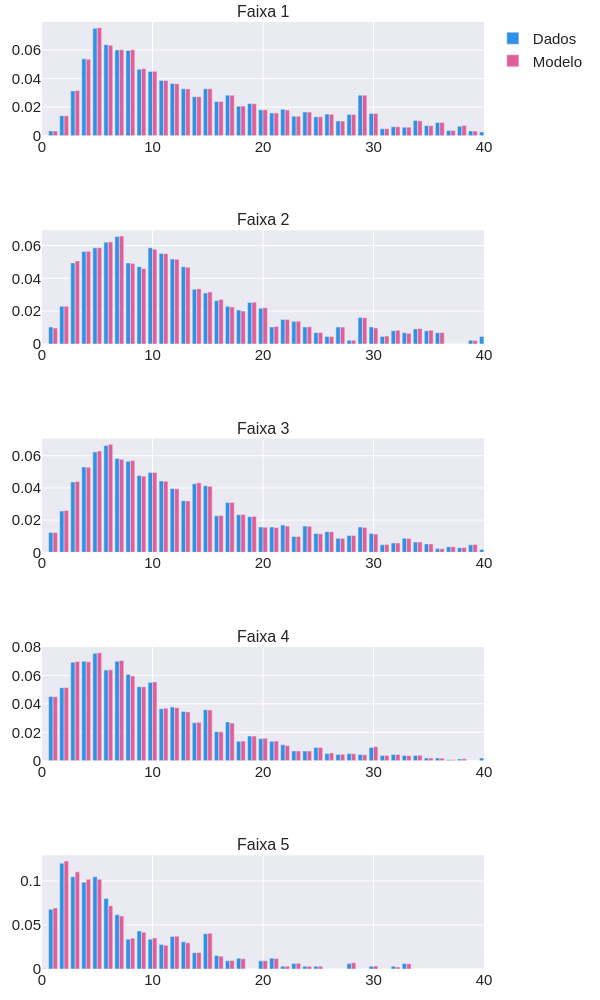
\includegraphics[scale= 0.4]{figuras/comparacao.png}
    \captionsetup{font=small,justification=justified}
    \caption*{Comparação de como fica a distribuição de graus comparando modelo com $p = 1.0$ com dados do POLYMOD, é possível ver todas as faixas foram bem no teste de comparação.\\Fonte: Autor}
    \label{fig:comparacao}
\end{figure}


\begin{figure}[H]
    \centering
    
    \captionsetup{font=normalsize,skip=0.8pt,singlelinecheck=on,labelsep=endash}
    \caption{Resultados da diferença absoluta entre a matriz de proporções de conexões entre faixas etárias encontradas no modelo e no POLYMOD}
    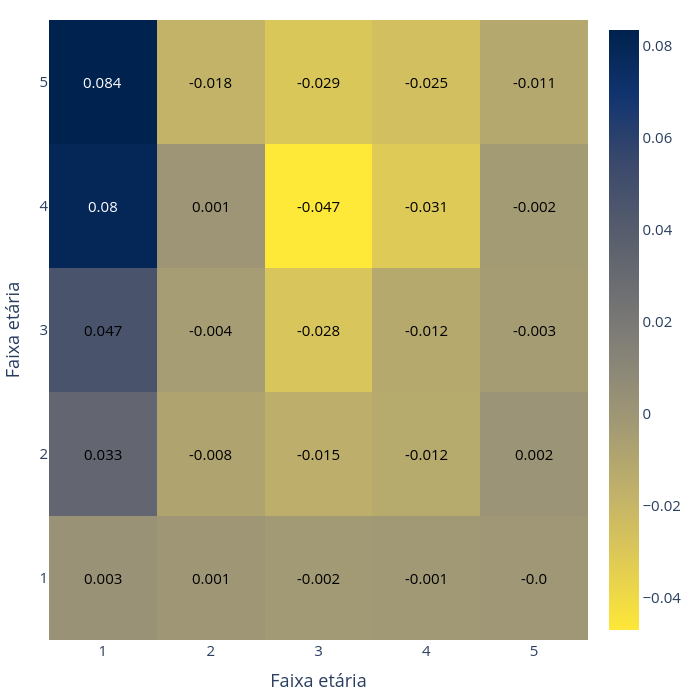
\includegraphics[scale= 0.4]{figuras/modelo.png}
    \captionsetup{font=small,justification=justified}
    \caption*{ A figura mostra a diferença absoluta entre a matriz de proporções de conexões entre as faixas etárias do modelo e do encontrado no POLYMOD; essa diferença se mantém constante independe do valor de $p$.}
    \label{fig:modelo}
\end{figure}

\begin{figure}[H]
    \centering
    \captionsetup{font=normalsize,skip=0.8pt,singlelinecheck=on,labelsep=endash}
    \caption{Variação da Correlação entre Agrupamento e Grau em função de $p$}
    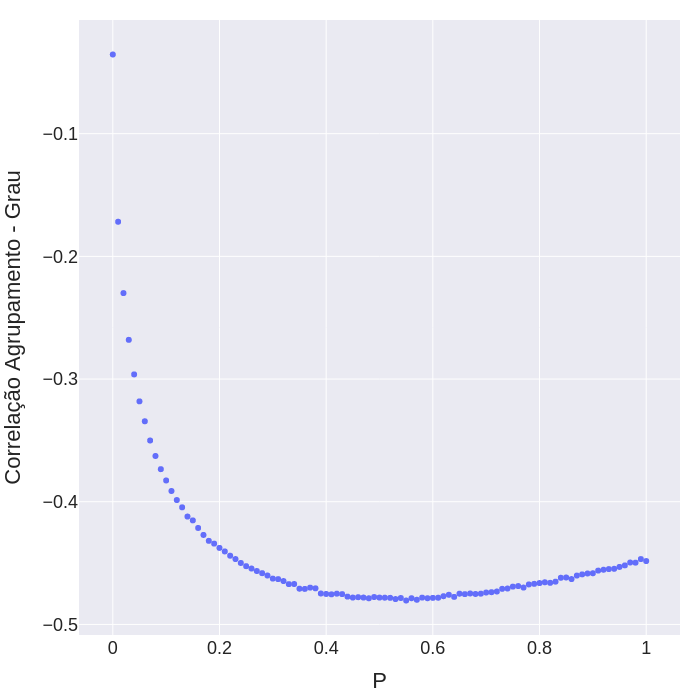
\includegraphics[scale= 0.45]{figuras/correlation.png}
    \captionsetup{font=small,justification=justified}   
    \caption*{Curva da correlação entre o grau e o agrupamento local em função de $p$. É possível ver que com o incremento de $p$ a correlação fica mais negativa, ou seja o algoritmo não consegue aumentar o agrupamento de nós com alto grau.\\Fonte: Autor}
    \label{fig:correlation}
\end{figure}

\section{Resultados do Modelo de Infecção}

Utilizando o Modelo de Configuração Ponderado, com entradas baseadas na distribuição de graus empírica, na distribuição de faixas etárias brasileiras e na distribuição de ligações entre faixas etárias do banco de dados do POLYMOD, os parâmetros do modelo de contágio foram obtidos da literatura ou calculados a partir do OpenDataSUS. As médias e desvios do tempo de contato entre indivíduos, também derivadas do POLYMOD, foram incorporadas como parâmetros do modelo. Com esses dados, iniciou-se a simulação da infecção.

A simulação acontece do dia 0 até o dia 465 iniciando com 10 nós infectados — para garantir que a simulação não termine cedo, caso tivesse menos nós infectados haveria a chance da infecção durar menos— 
no compartimento Exposto e todos os outros sítios como Suscetíveis. A vacinação ocorre no dia 100, nesse dia são aplicadas vacinas para uma fração $f$ da rede para sítios no compartimento Suscetível, Exposto, Recuperado ou Assintomático dado um critério de prioridade que é determinado pelo valor das centralidades introduzidas anteriormente. Se o indivíduo não estiver apto a ser vacinado no dia e após todos os aptos serem vacinados ainda existirem vacinas sobrando, então se ele atingir um dos compartimentos aptos, ele será vacinado.


No caso de redes ponderadas nos vértices e nas arestas, dois tipos de peso dos nós foram considerados: 
a probabilidade do nó ser assintomático e a probabilidade dele morrer. 
Para centralidades que originalmente não utilizam ponderação dos nós, apenas nas arestas, utilizamos a seguinte transformação no peso das arestas. 
\begin{equation}
    Z_{\nu,\mu} = w_{\nu,\mu}\cdot(\Theta_\nu + \Theta_\mu).
\end{equation}
O valor de $\Theta_\nu$ e $\Theta_\mu$, que são os pesos de cada vértice, e das centralidades com ponderação dos nós será feito em duas abordagens diferentes: Altruísta e a Individualista. A Altruísta será calculando 
a centralidade do nó $\nu$ considerando o risco do nó $\nu$ infectar outros nós e eles morrerem, ou seja $\Theta_\nu = \alpha_f(\nu)$,$\Theta_\mu = \tau_f(\mu)$ . Por outro lado, na abordagem Individualista, o cálculo da centralidade do nó $\nu$ considera o risco do nó $\nu$ ser infectado por um vizinho e morrer, ou seja $\Theta_\nu = \tau_f(\nu)$,$\Theta_\mu = \alpha_f(\mu)$. Conferir \ref{tabela:probabilidades_transicao_adaptada}.  

Após a 
simulação do modelo epidemiológico 
na rede gerada pelo Modelo de Configuração adaptado,
foi observado que após o dia 100 a infecção estabilizava e esse seria o dia da vacinação. 
Deste modo, simula-se a situação real na qual a vacina só se tornou disponível após a COVID-19 já ter se espalhado por todo o mundo. Anteriormente a esse dia a rede se comporta, para $p = 0$ (com agrupamento médio de 0.01), de acordo com as Figuras \ref{fig:pre_vacina} e \ref{fig:pre_vacina_mortos}
, nas quais foi feita uma média com 400 simulações.

A Figura \ref{fig:pre_vacina} mostra a evolução da epidemia, em que pode-se observar que a proporção de indivíduos suscetíveis diminui rapidamente até o dia 25
para posteriormente aumentar e atingir um estado de estabilidade. A fração de indivíduos infectados (a soma da fração de assintomáticos com a de sintomáticos) aumenta até atingir um pico, com  30\% da população total sendo infectada simultaneamente, seguido por um declínio. Finalmente, a fração de indivíduos recuperados aumenta até que 58\% da população esteja nesse estado, estabilizando posteriormente. 

A Figura \ref{fig:pre_vacina_mortos} mostra a evolução  da fração de mortos e a fração de hospitalizados. Observa-se que o número máximo de hospitalizados observado foi cerca de 0.46\% da rede, enquanto o número de mortos cresce indefinidamente. Neste trabalho, não consideramos a capacidade do sistema hospitalar, pois neste caso, precisaríamos de informações sobre a taxa de recuperação e de morte de sintomáticos que precisariam ser internados e não foram por falta de leitos, que não são facilmente determinadas.   

\begin{figure}[H]
    \centering
    \captionsetup{font=normalsize,skip=0.8pt,singlelinecheck=on,labelsep=endash}
    \caption{Fração de Suscetíveis, Infectados e Recuperados antes da aplicação de qualquer estratégia de vacinação}
    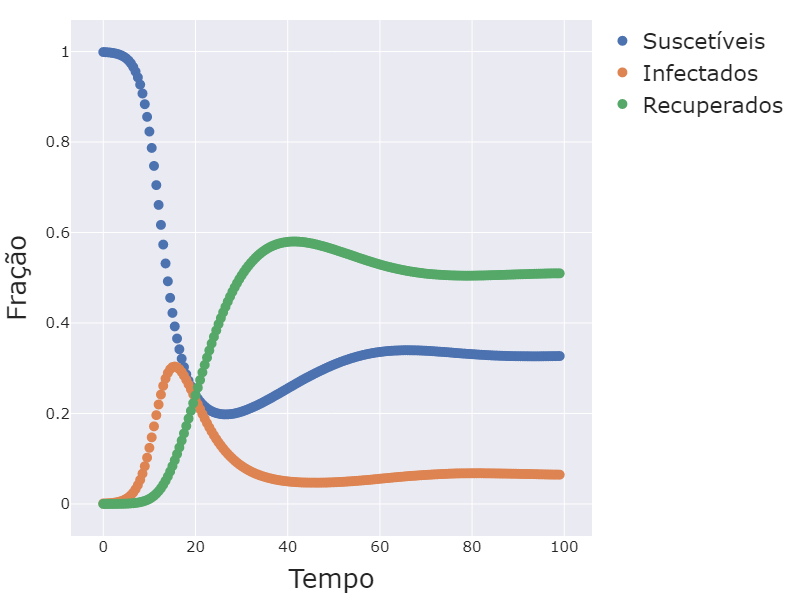
\includegraphics[scale= 0.4]{figuras/pre_vacina_nponderado.png}
    \captionsetup{font=small,justification=justified}
    \caption*{Resultados antes da aplicação de qualquer 
    estratégia de vacinação para uma rede $N$ = 10000 com $p $ = 0 após 400 realizações. Inicialmente, a proporção de suscetíveis diminui rapidamente, seguida por um aumento e estabilização. A fração de infectados atinge um pico, afetando 
    40\% da população, e depois diminui. Paralelamente, a proporção de recuperados aumenta e estabiliza em 71\% da população.}
    \label{fig:pre_vacina}
\end{figure}

\begin{figure}[H]
    \centering
    \captionsetup{font=normalsize,skip=0.8pt,singlelinecheck=on,labelsep=endash}
    \caption{Fração de Hospitalizados e Mortos antes da aplicação de qualquer estratégia de vacinação}
    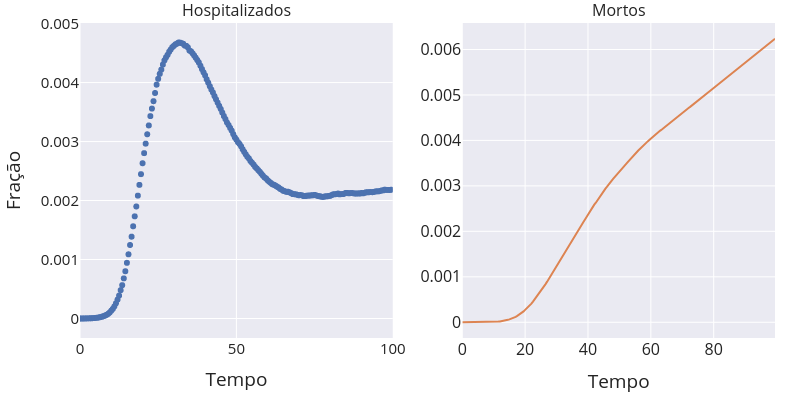
\includegraphics[scale= 0.5]{figuras/pre_vacina_mortos_nponderado.png}
    \captionsetup{font=small,justification=justified}
    \caption*{Simulações foram feitas para uma rede $N$ = 10000 com $p $ = 0 após 400 realizações. O gráfico mostra que a Fração de Hospitalizados chega a um limite máximo de pessoas que podem estar no estágio ao mesmo tempo enquanto que a fração de mortos cresce indefinidamente até chegar em aproximadamente 0.6\% da rede.}
    \label{fig:pre_vacina_mortos}
\end{figure}

Com o aumento de $p$ surgem diferenças com o comportamento da infecção
; a Figura~\ref{fig:pre_vacina_mortos_p} mostra 
que a rede tem uma quantidade menor de mortos, contudo a infecção demora mais para crescer, decair e estabilizar, ou seja o agente permanece mais tempo na rede, isso se deve, provavelmente, ao fato de que com o maior agrupamento a infecção fica presa em regiões com alto agrupamento e tem muita dificuldade em avançar para outras regiões da rede.

\begin{figure}[H]
    \centering
    \caption{Fração de Expostos e Mortos antes da aplicação de qualquer estratégia de vacinação para diferentes valores de $p$}
    \vspace{5pt}
    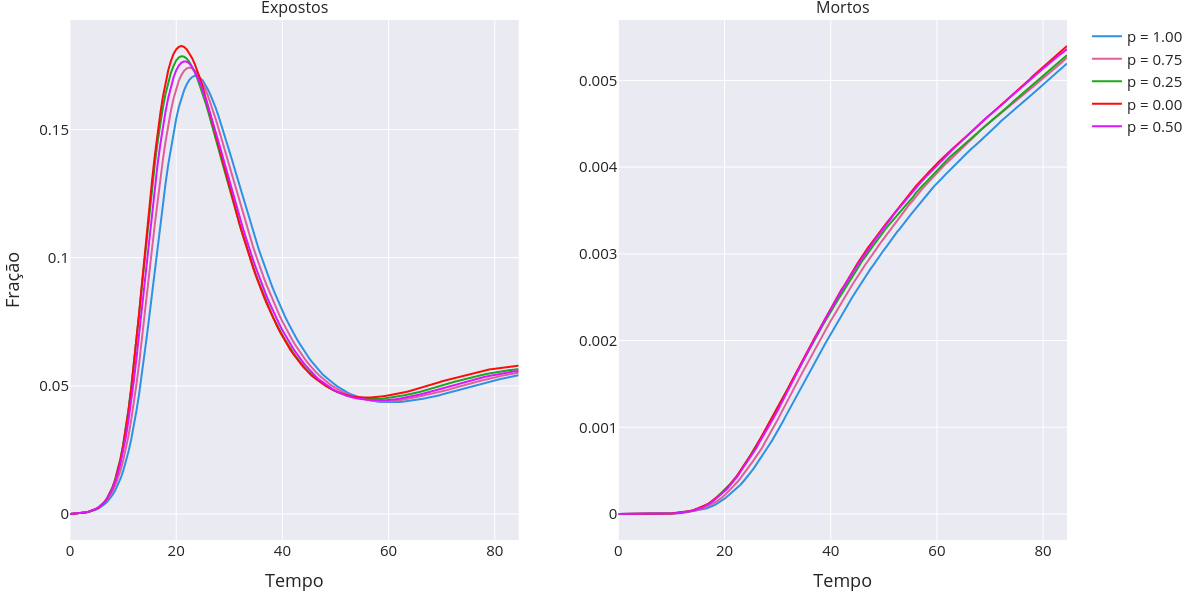
\includegraphics[width=\textwidth]{figuras/pre_vacina_mortos_p_nponderado.png}
    \captionsetup{font=small,justification=justified}
    \caption*{Resultados para fração de
    Expostos e Mortos em função do tempo antes da aplicação de qualquer estratégia de vacinação para uma rede $N$ = 10000 para diferentes valores de $p$. Quanto maior o $p$ menor a fração de mortos e o número de Expostos tende a demorar a estabilizar, resultado das conexões entre faixas.}
    \label{fig:pre_vacina_mortos_p}
\end{figure}

Para finalizar, fizemos a comparação entre como a 
infeção se espalha nos primeiros 100 dias no caso ponderado e não ponderado.
Nesse caso não houve uma diferença significativa entre o avanço da infecção.
Assim como a Figura \ref{fig:compara_ponderado_nponderado} mostra para Sintomáticos que a diferença é pouco perceptível, também isso é visível para qualquer outro estado. 
Apesar disso, 
foi
feita a análise das centralidades comparando caso ponderado e não ponderado, porém no caso da infecção pré-vacina não há diferença o que acarreta numa simplificação do modelo o que favorece o tempo computacional dos algoritmos.

\begin{figure}[H]
    \centering
    \captionsetup{font=normalsize,skip=0.8pt,singlelinecheck=on,labelsep=endash}
    \caption{Comparação entre a ponderação nas arestas e sem ponderação}
    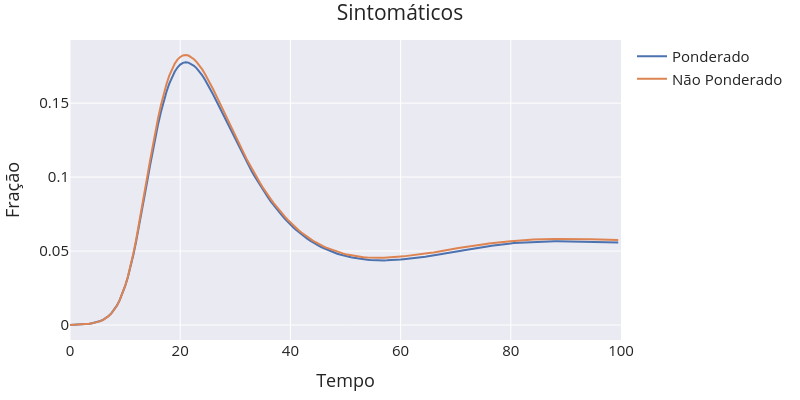
\includegraphics[scale= 0.5]{figuras/compara_ponderado_nponderado.png}
    \captionsetup{font=small,justification=justified}
    
    \caption*{Nesse gráfico mostra a diferença sútil entre o caso não ponderado  nas arestas e ponderado nas arestas para os Sintomáticos. 
    }
    \label{fig:compara_ponderado_nponderado}
\end{figure}

\section{Resultado das Estratégias de Vacinação}

A simulação foi feita considerando que após decorridos 100 dias, a vacina foi aplicada considerando como ordem de prioridade diversas estratégias seguindo as centralidades em redes apresentadas anteriormente, e foram propostas 4 ou medidas que são a probabilidade do sítio contaminar seus vizinhos e ser hospitalizado $PH$, a probabilidade dele contaminar os vizinhos dado que é assintomático $PHA$, a probabilidade dele ser contaminado e morrer $PM$ e a probabilidade dele matar os vizinhos dado que é assintomático $PMA$. Ao final foram coletadas 
três métricas de desempenho das estratégias: 
a soma de todos os tempos de hospialização de todos os indivíduos da rede $T_H$, a fração de mortos $F_M$ e fração de indivíduos 
vacinados 
necessária para extinguir a doença $F_I$.
Assim para cada 
uma dessas métricas
foi feito um \textit{ranking} mostrando para as melhores centralidades.
Como os valores de $T_H$ e $F_M$ dependem de $f$, 
a fração de vacinados, 
a métrica utilizada foi a área abaixo do gráfico das curvas de $T_H$ e $F_M$ em função de $f$.
Para determinar qual centralidade apresentou o melhor desempenho geral, foi calculada a média dos valores normalizados das três métricas para cada centralidade. A normalização foi feita ajustando os valores de cada métrica para um intervalo entre 0 e 1, de modo que os valores mais baixos fossem transformados para 0 e os mais altos para 1.
A qualidade 
do desempenho
de cada centralidade 
depende
da estrutura da rede, ou seja, com a alteração de $p$ o \textit{ranking} 
poderá ser diferente e  
podem existir diferentes melhores estratégias, 
sendo, neste caso, necessário estimar os valores de $p$ da rede real para saber qual seria a melhor estratégia
a ser utilizada na prática. 


Para o caso sem ponderação, a Figura \ref{fig:resultados_metricas} ilustra 
como ficaram os resultados para $p = 0$ e $p = 1$ mostrando 4 
estratégias: 
o caso aleatório, idade, a melhor na métrica e a melhor na média. 
Quando o gráfico apresenta apenas 3 curvas significa que a melhor na métrica é a mesma para melhor na média. Esse esquema será repetido na Figura \ref{fig:resultados_metricas_ponderado}.
Para o leitor interessado, os resultados de todas as centralidades 
(29 para caso não ponderado e 65 para caso não ponderado) 
estão no Apêndice 1.

É possível perceber que em todas as métricas e mudando o valor de $p$ a idade não foi a melhor estratégia, um resultado importante é que para extinguir a doença seria necessário vacinar cerca de 80\% da população, entretanto na melhor estratégia foram necessários apenas 32\% para extinguir a doença. Porém é notável que para uma fração menor de 15\% da rede vacinada a idade foi muito boa em comparação às melhores. 
Essa comparação é feita pois foi a principal estratégia utilizada pelos governos.


\begin{figure}[H]
    \centering
    \captionsetup{font=normalsize,skip=0.8pt,singlelinecheck=on,labelsep=endash}
    \caption{Gráfico para cada métrica por fração de vacinados para $p = 0$ e $p = 1.0$ sem ponderação nas arestas}
    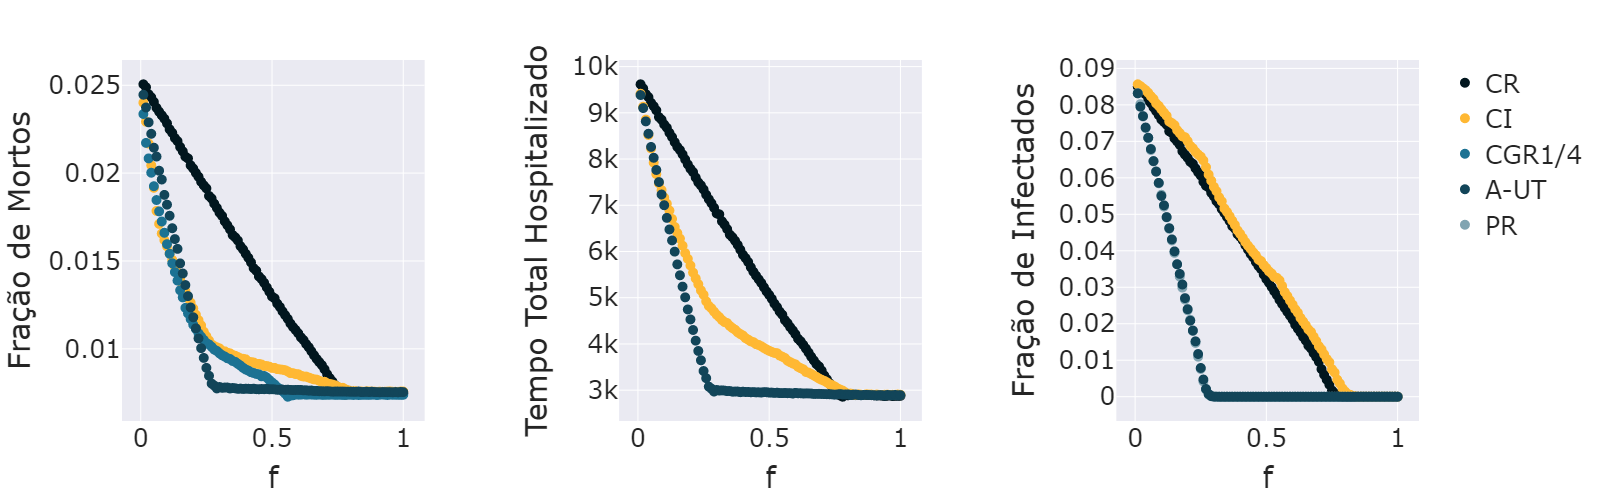
\includegraphics[scale= 0.3]{figuras/compara_p_f_nponderado_0.0.png}
    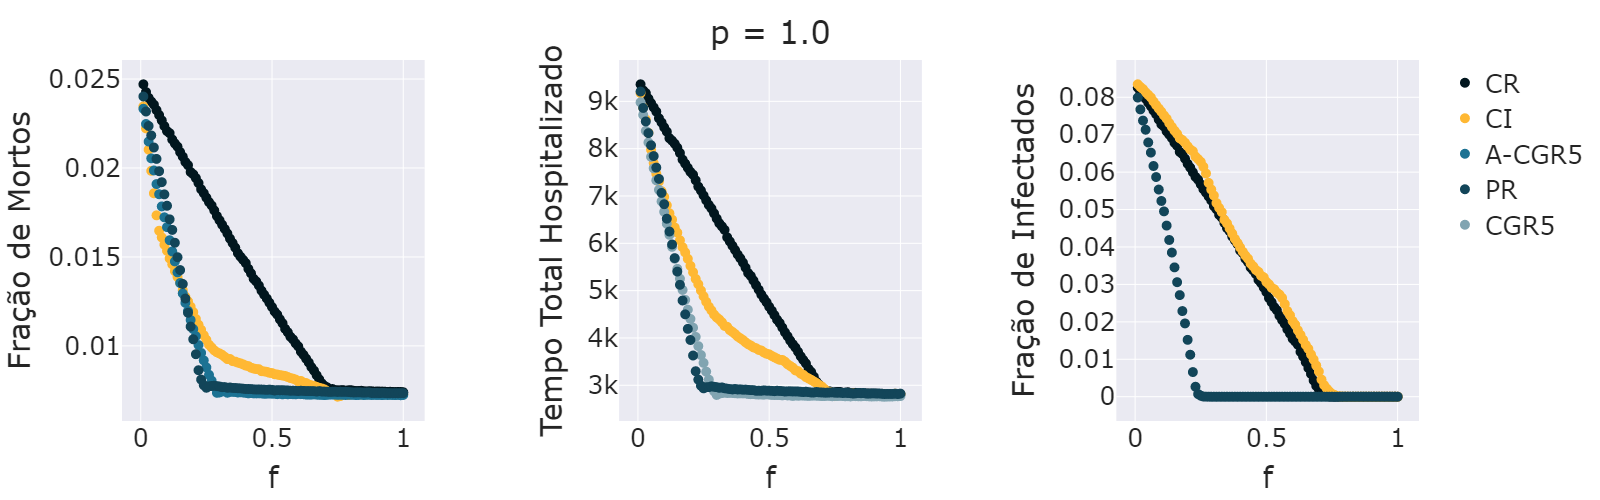
\includegraphics[scale= 0.3]{figuras/compara_p_f_nponderado_1.0.png}
    \captionsetup{font=small,justification=justified}
    
    \caption*{Comparação de cada métrica, no para os dois primeiros gráficos foi utilizado  critério da integral enquanto no último foiavaliado o valor de $f$ quando a curva toca o 0. Comparando as melhores decada métrica e a média contra a estratégia aleatória (CR) e  idade (CI). Para $p = 0$, a melhor estratégia 
    na média
    foi a Utilidade com abordagem Altruísta (A-UT) no caso da Fração de Mortos a melhor estratégia foi a Gravidade com expoente 1/4 (CGR1/4) já na Fração de Vacinados foi o \textit{PageRank} (PR). No caso $p = 1.00$ o melhor em média foi o  \textit{PageRank}, na Fração de Mortos a Gravidade com abordagem Altruísta com expoente 5 (A-CGR5) e a Individualista (CGR5) foi a melhor na Fração de Vacinados.}
    \label{fig:resultados_metricas}
\end{figure}

\begin{figure}[H]
    \centering
    \captionsetup{font=normalsize,skip=0.8pt,singlelinecheck=on,labelsep=endash}
    \caption{Gráfico para cada métrica por fração de vacinados para $p = 0$ e $p = 1.0$ com ponderação nas arestas}
    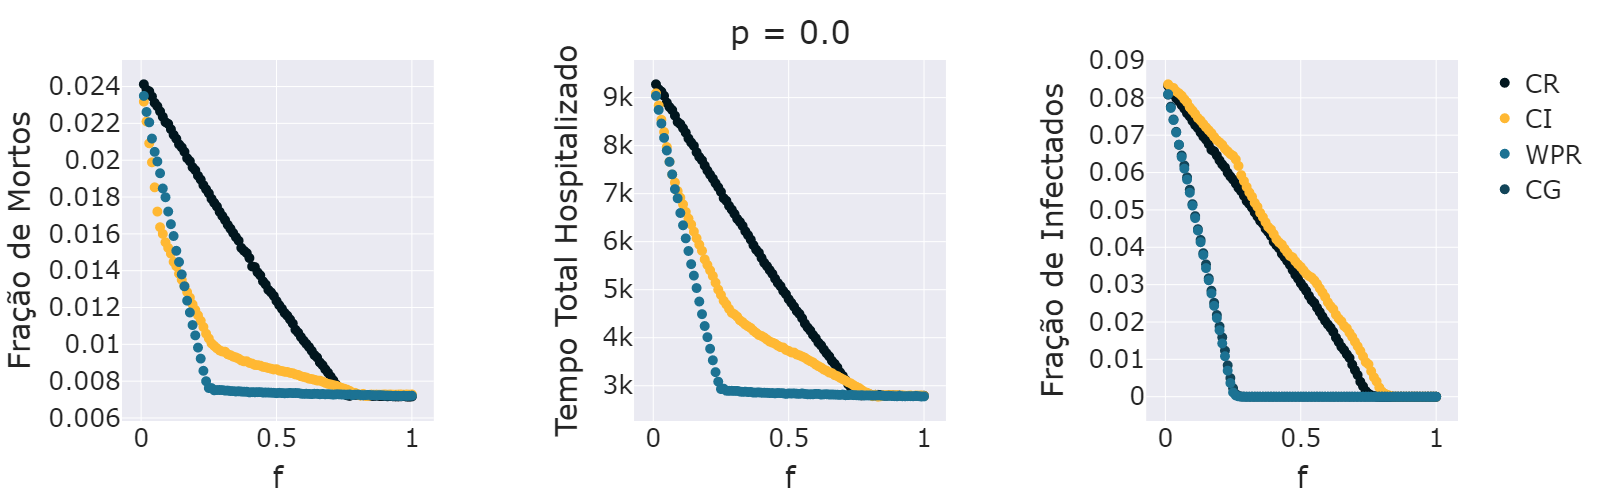
\includegraphics[scale= 0.3]{figuras/compara_p_f_ponderado_0.0.png}
    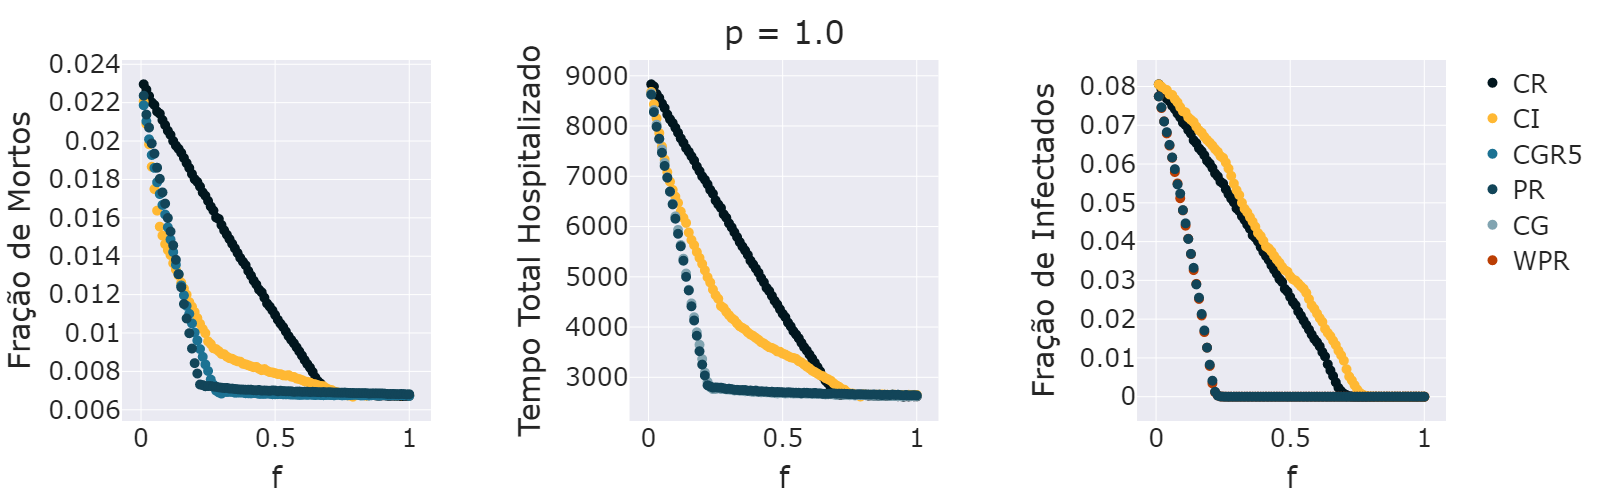
\includegraphics[scale= 0.3]{figuras/compara_p_f_ponderado_1.0.png}

    \captionsetup{font=small,justification=justified}
    
    \caption*{Comparação de cada métrica, no para os dois primeiros gráficos foi utilizado  critério da integral enquanto no último foiavaliado o valor de $f$ quando a curva toca o 0. Comparando as melhores decada métrica e a média contra a estratégia aleatória (CR) e  idade (CI). Para $p = 0$, a melhor estratégia 
    na média
    foi o \textit{PageRank} com pesos nas arestas (WPR) e foi a melhor em Frção de Mortos e Tempo Hospitalizado, enquanto que no último foi o Grau (CG). No caso $p = 1$ o melhor na média foi o \textit{PageRank} enquanto que o melhor na Fração de Mortos foi a Gravidade com expoente 5, o tempo total hospitalizado foi o Grau e na Fração de Vacinados foi o \textit{PageRank} ponderado nas arestas. }
    \label{fig:resultados_metricas_ponderado}
\end{figure}

Embora os gráficos forneçam uma indicação preliminar da diferença entre a melhor estratégia em termos de 
uma determinada métrica de desempenho
e do desempenho médio, é fundamental realizar uma avaliação para determinar se existe uma diferença significativa entre 
os \textit{rankings} para as diferentes métricas. Nesse caso, 
foi
feita a correlação de Spearman entre 
os \textit{rankings}
das métricas. A Figura \ref{fig:Spearman} mostra o valor da correlação para diferentes valores de $p$ para o caso não ponderado e ponderado. É possível ver que as duas métricas mais distintas entre si são $F_M$ e $F_I$ mostrando que a métrica que foca em diminuir a mortalidade 
não necessariamente previne a espalhamento da doença. 
Vale ressaltar, que com o incremento de $p$, $F_M$ e $T_H$ se tornam mais próximas.
Por fim, existe uma diferença no caso ponderado, na qual as métricas são mais próximas entre si, principalmente a $F_M$ e $T_H$.

\begin{figure}[H]
    \centering
    \captionsetup{font=normalsize,skip=0.8pt,singlelinecheck=on,labelsep=endash}
    \caption{Correlação entre o ranqueamento entre cada métrica}
    
    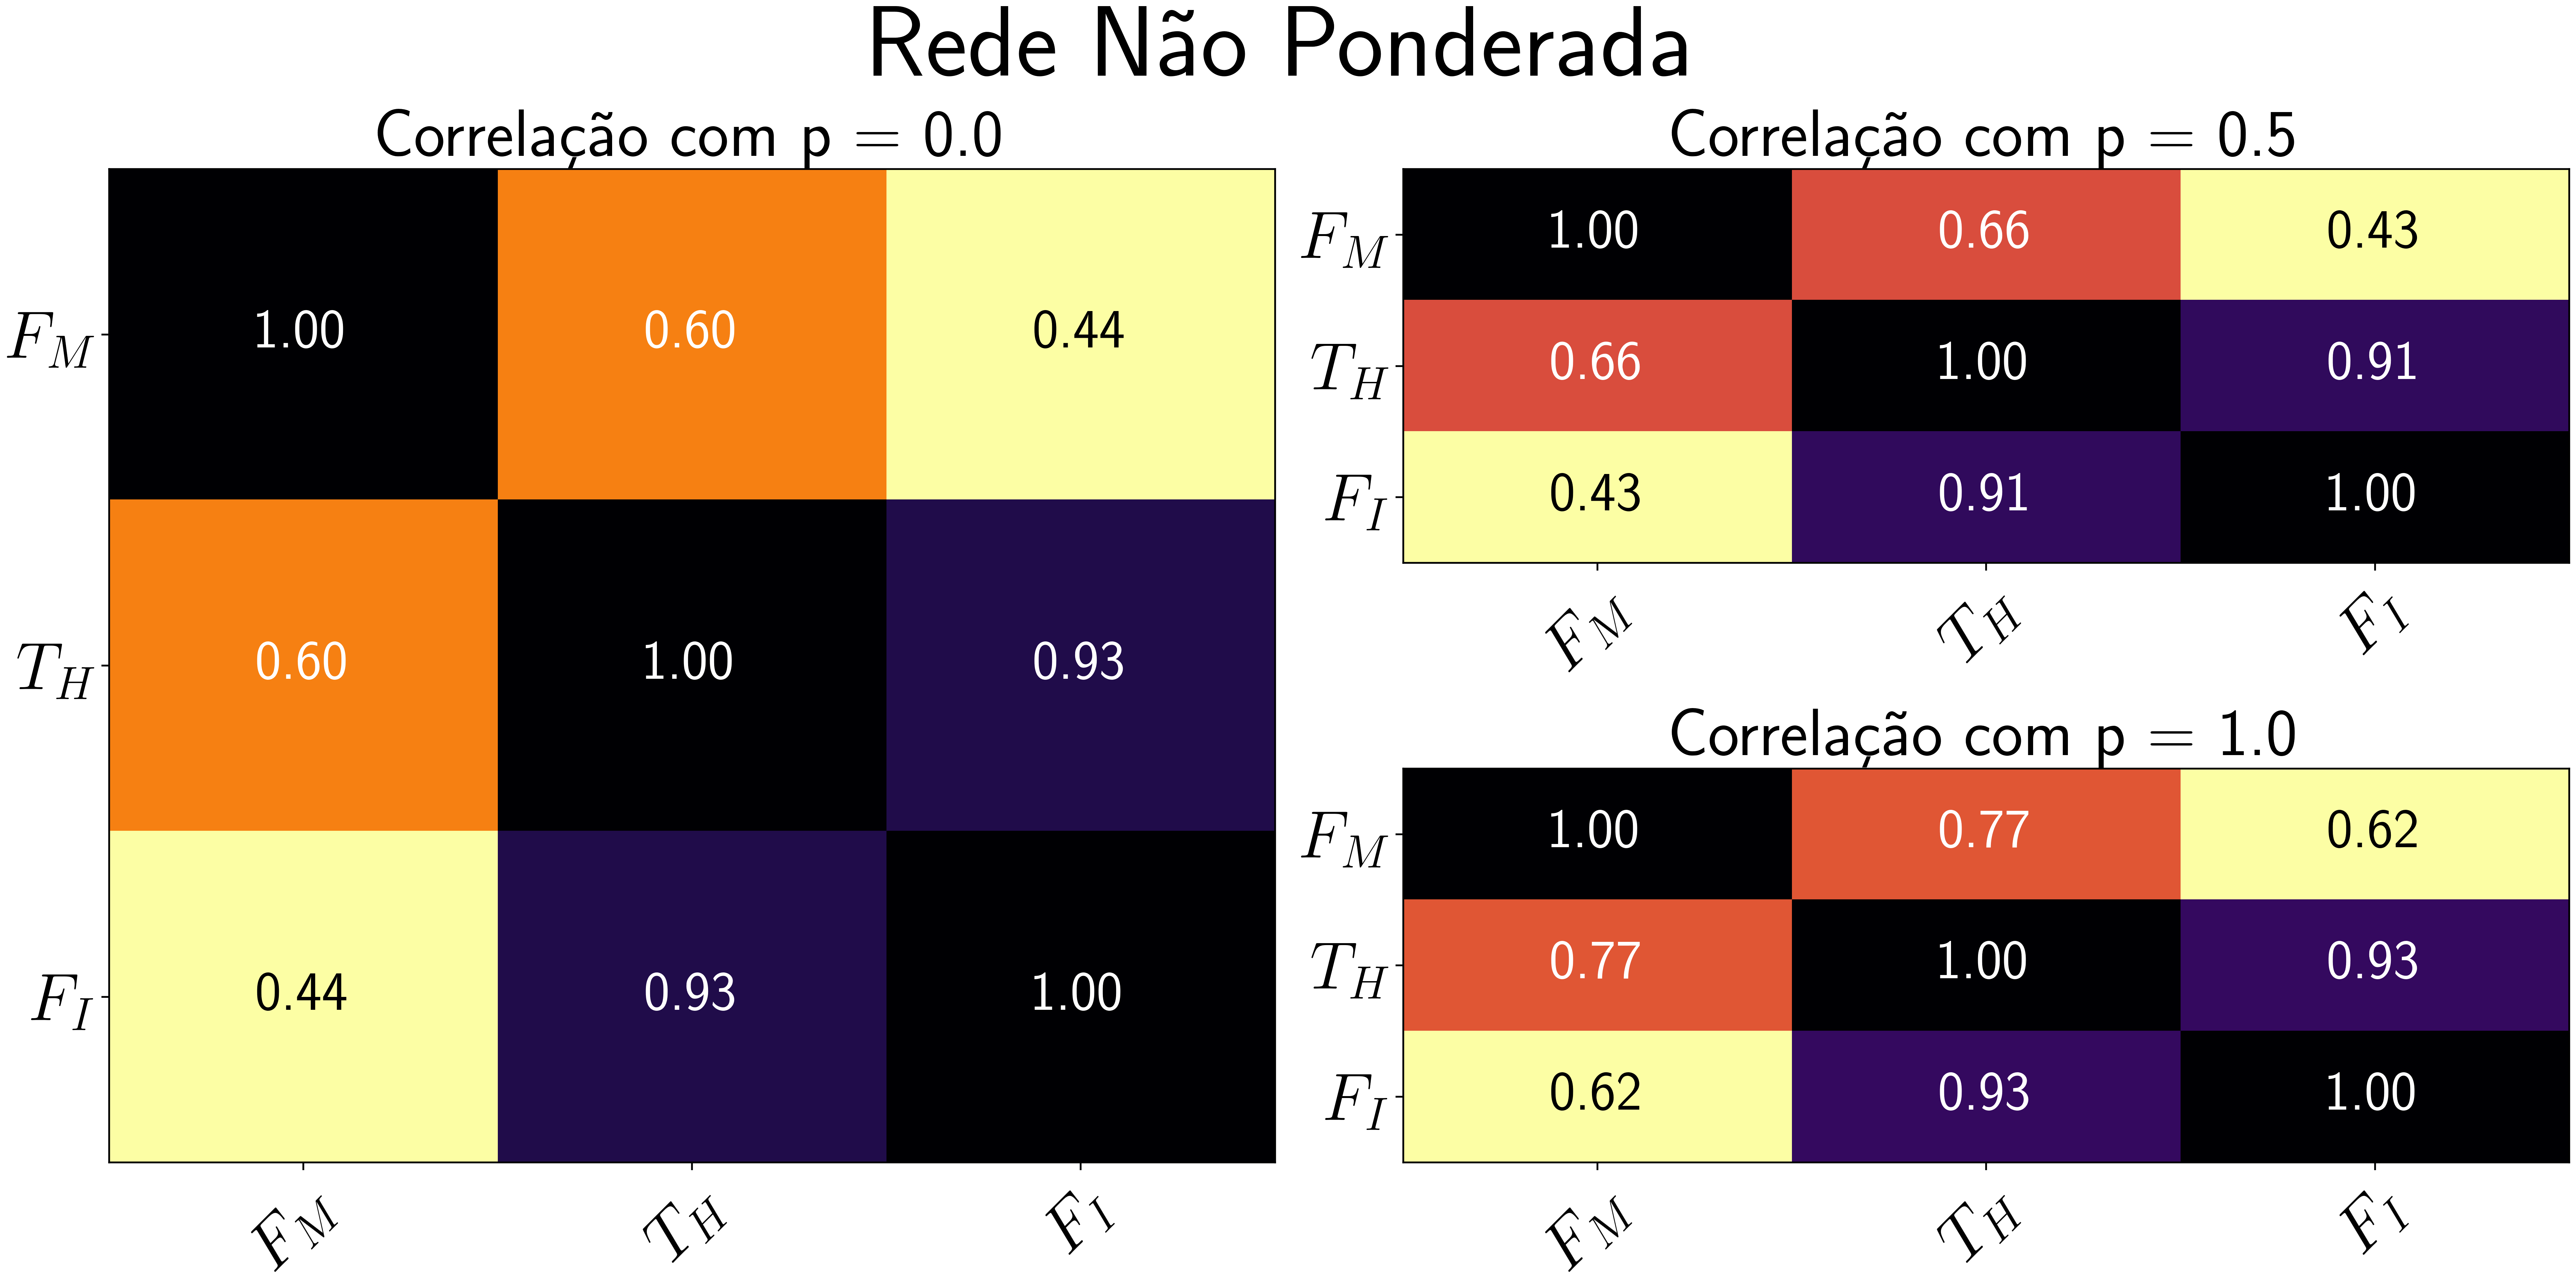
\includegraphics[scale= 0.4]{figuras/corr_p.png}
    \\
    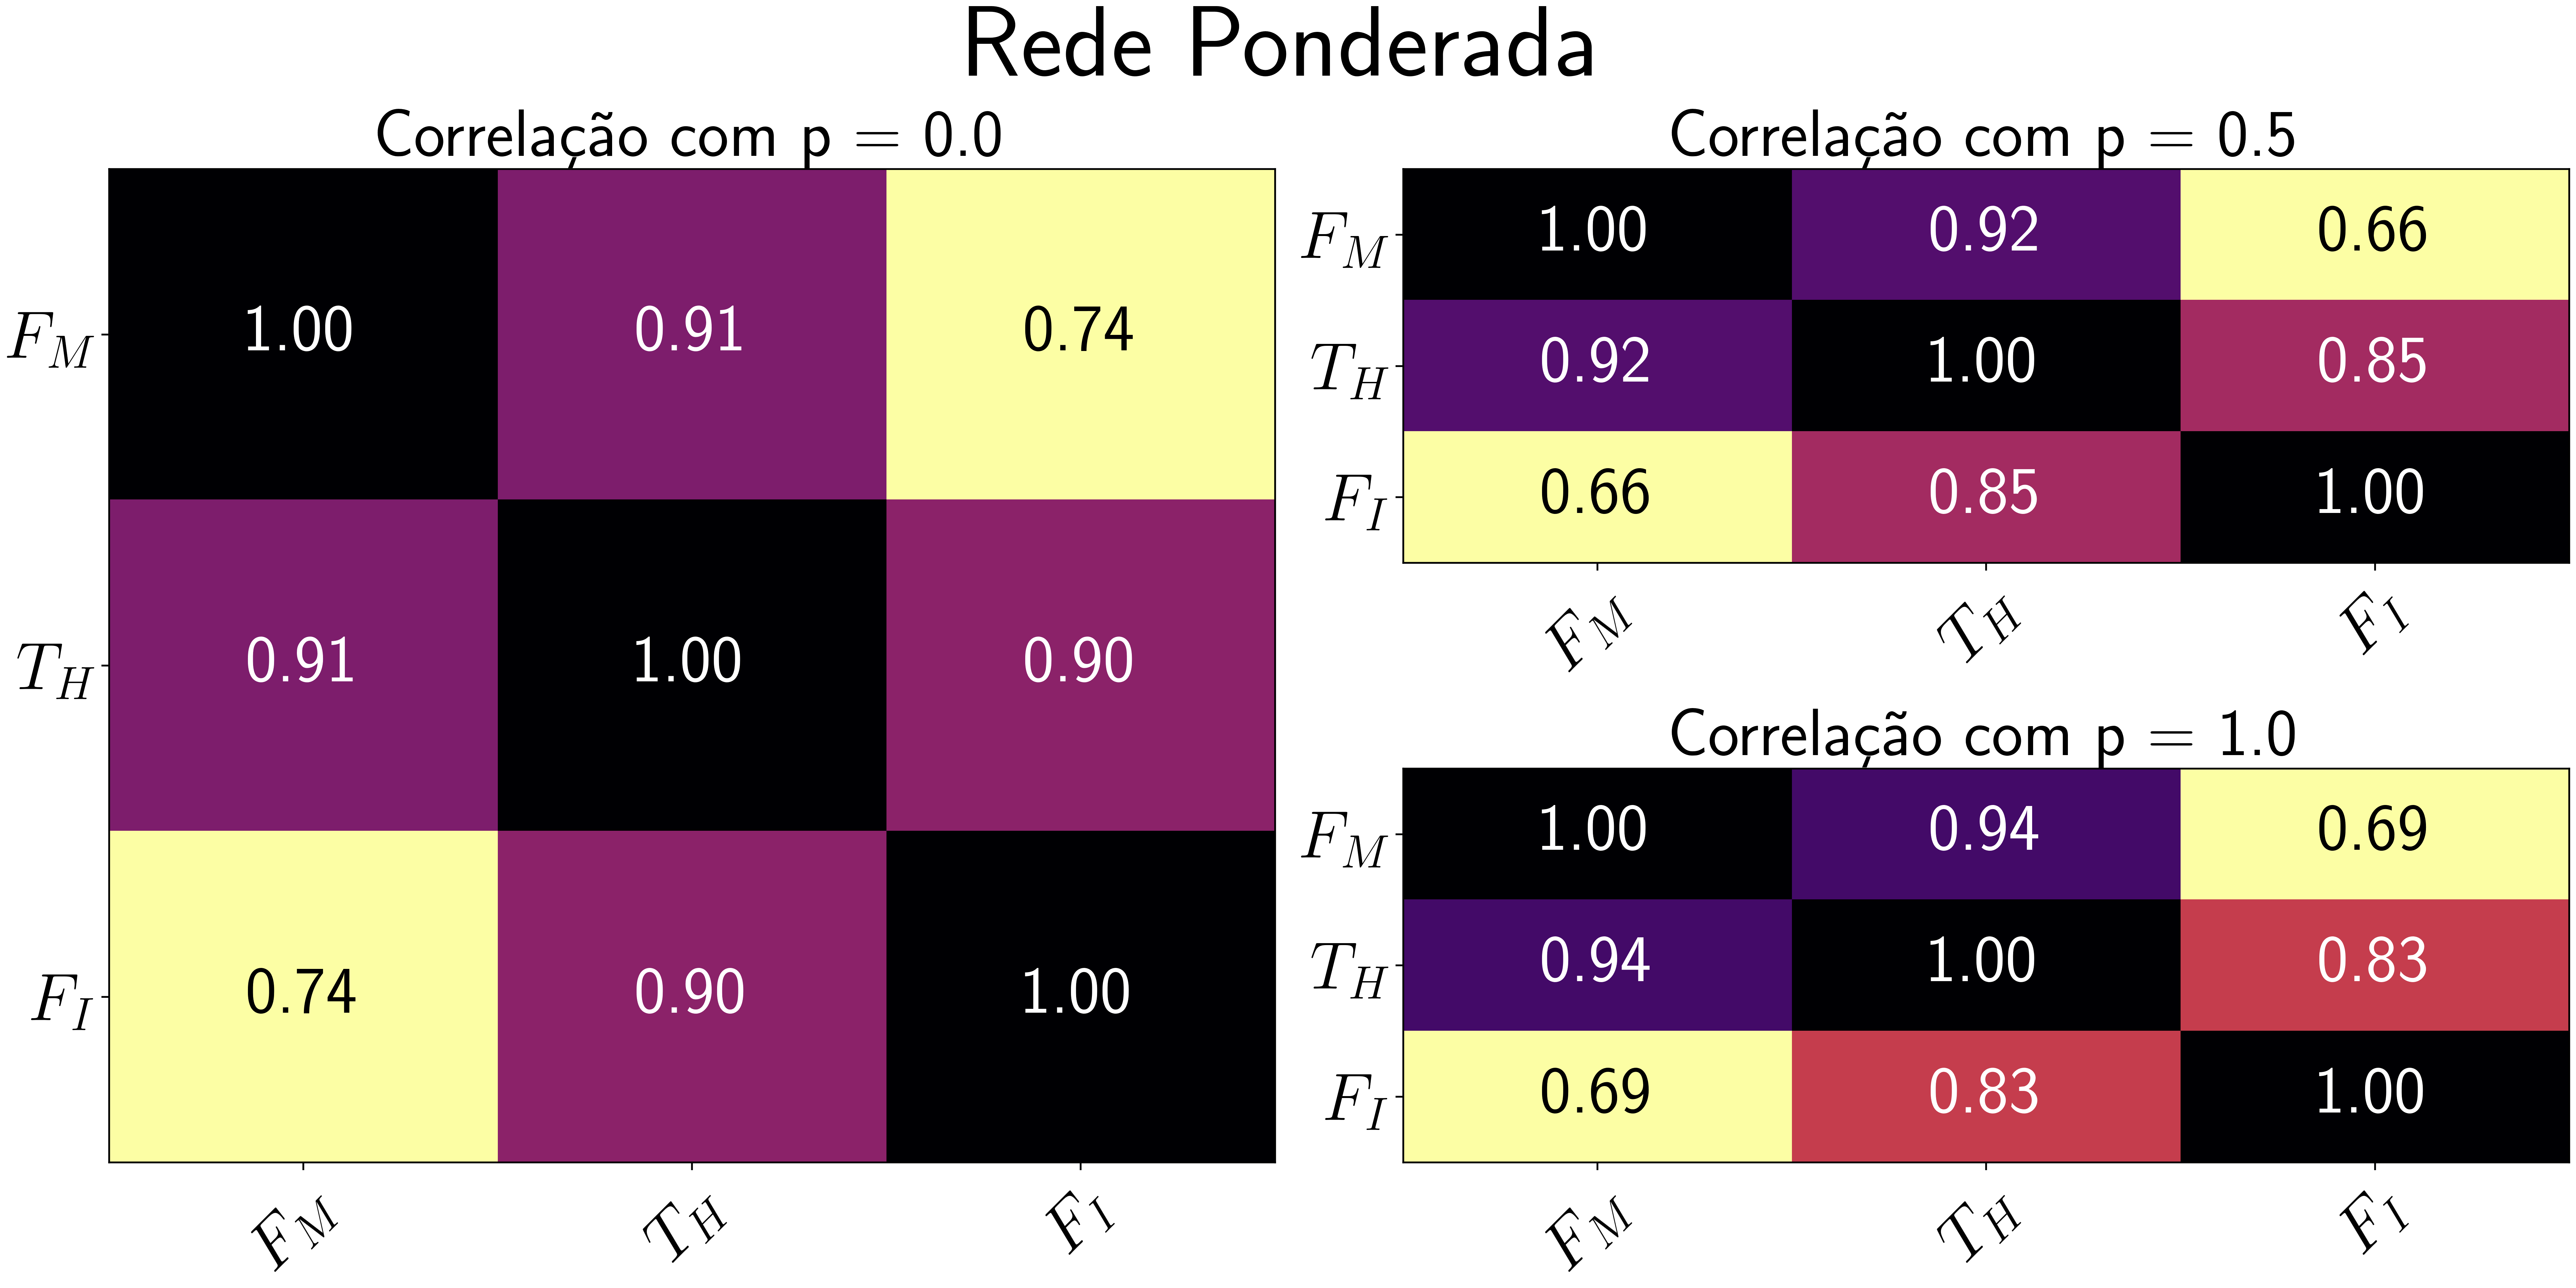
\includegraphics[scale= 0.4]{figuras/corr_p_ponderado.png}
    \captionsetup{font=small,justification=justified}
    \caption*{A correlação entre o ranqueamento das métricas mostra que $F_I$ e $F_M$ são as mais diferentes, entretanto com o incremento de $p$ a diferença diminui, para ambos os casos de rede ponderada nas arestas e não ponderada. Além disso na rede ponderada a correlação é muito maior que a não ponderada.}
    \label{fig:Spearman}
\end{figure}

Como mostrado pela Figura \ref{fig:Spearman}, as relações entre métricas mudam com o incremento de $p$, assim o próprio \textit{ranking} das centralidades muda com a variação deste parâmetro. A Figura \ref{fig:Spearman_p} mostra a correlação de Spearman do \textit{ranking} das centralidades para cada par de valores para $p$, considerando rede não ponderada e ponderada. É possível ver que para o caso não ponderado no geral existe uma alta correlação entre os pares, tanto para $p = 0.0$ quanto para $p = 1.00$. Isso mostra que o posicionamento das estratégias é bastante estável com o aumento do agrupamento tanto no caso ponderado quanto não ponderado. Isso é bastante útil pois não foi medido o agrupamento da rede real de contatos entre pessoas e com essa estabilidade não se torna tão necessário estimar esse valor.

\begin{figure}[H]
    \centering
    \captionsetup{font=normalsize,skip=0.8pt,singlelinecheck=on,labelsep=endash}
    \caption{Correlação entre o ranqueamento de cada métrica para cada agrupamento}
    
    \includegraphics[scale= 0.4]{figuras/compara_agrupamento_nponderado.png}
    \\
    \includegraphics[scale= 0.4]{figuras/compara_agrupamento_ponderado.png}
    \captionsetup{font=small,justification=justified}
    \caption*{Para cada métrica foi 
    feita uma correlação de Spearman entre os 5 valores de $p$ tanto para ponderação nas arestas quanto sem ponderação. Em ambos os casos mostra-se que a classificação se altera pouco o que é útil pois estimar o agrupamento de uma rede de contatos real é custoso.}
    \label{fig:Spearman_p}
\end{figure}

Anteriormente foram apresentadas as centralidades e as suas versões utilizando ponderamento nas arestas, contudo a utilização da forma ponderada tem um custo computacional bastante considerável, portanto foi avaliado como a métrica foi em comparação com a sua versão ponderada considerando a diferença relativa entre o valor na métrica com ponderação em relação ao valor sem considerar ponderação. A Figura \ref{fig:compara_pesos} mostra como ficou a comparação para dois casos de agrupamento $p = 0$ e pode se perceber que várias métricas não foram bem com o incremento da ponderação nas arestas, principalmente a Utilidade que para $F_I$ teve uma perca de 100\%, mas algumas conseguiram se beneficiar, mas no geral 
a maioria teve uma queda de desempenho ao se considerar os pesos nas arestas.

\begin{figure}[H]
    \centering
    \captionsetup{font=normalsize,skip=0.8pt,singlelinecheck=on,labelsep=endash}
    \caption{Diferença relativa da centralidade com e sem peso nas arestas}
    
    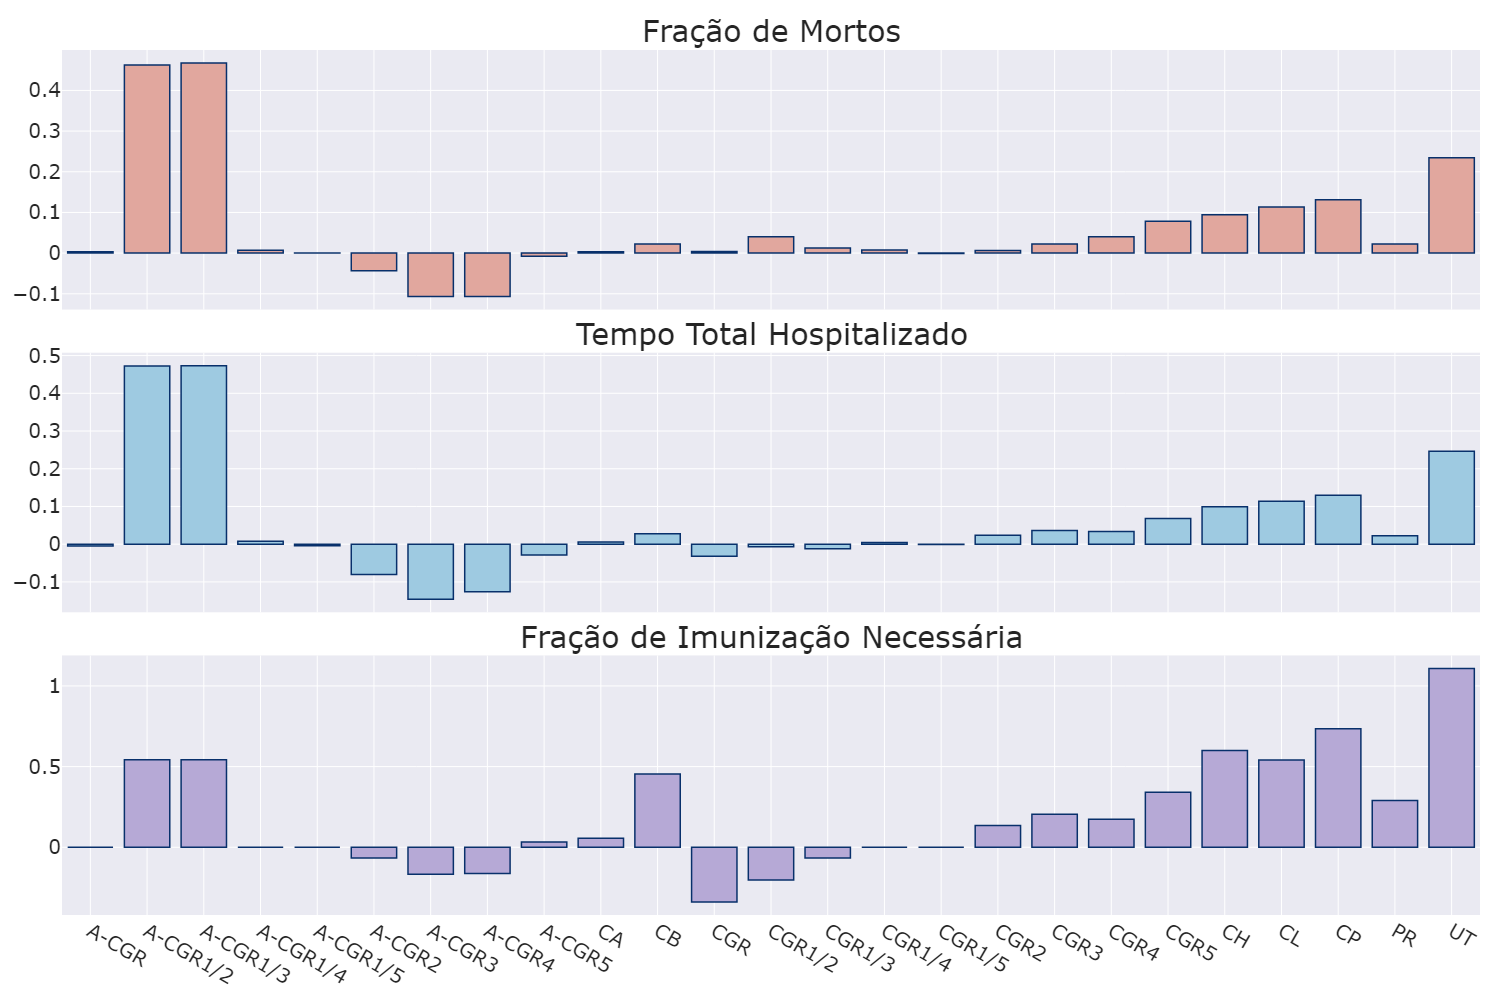
\includegraphics[scale= 0.3]{figuras/compara_pesos_0.0.png}
    \\
    \captionsetup{font=small,justification=justified}
    \caption*{Diferença relativa entre ponderação nas arestas: em todas as métricas a diferença foi irrelevante ou houve uma piora considerável, não utilizá-las reduz o custo computacional do cálculo das centralidades.}
    \label{fig:compara_pesos}
\end{figure}

Diferente da comparação entre o ponderado e não ponderado, a comparação entre Individualista e Altruísta pelo erro relativo é consenso, como mostra a Figura \ref{fig:compara_altruismo}, que o Individualista foi muito pior que a abordagem Altruísta pois ou os valores eram bastante parecidos ou havia uma piora muito grande. 
No caso da rede ponderada, muitas métricas pioraram e nas outras havia pouca mudança, já na rede não ponderada 
foi observado 
o contrário.
\begin{figure}[H]
    \centering
    \captionsetup{font=normalsize,skip=0.8pt,singlelinecheck=on,labelsep=endash}
    \caption{Diferença relativa entre abordagem Individualista e Altruista}
    
    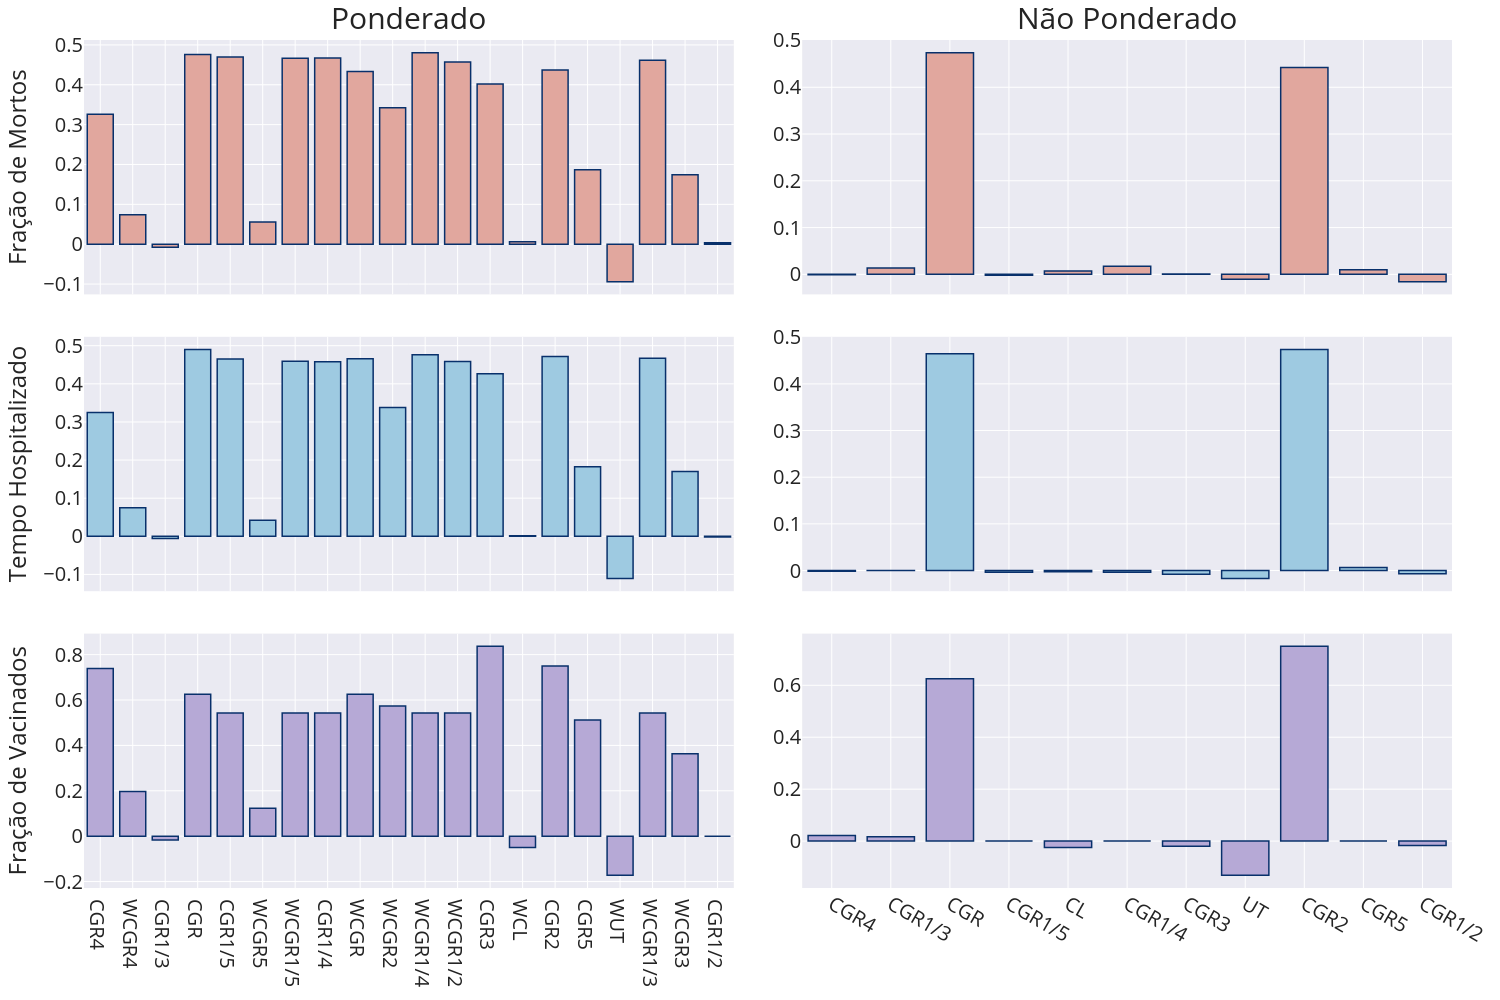
\includegraphics[scale= 0.3]{figuras/compara_altruismo_0.0.png}
    \captionsetup{font=small,justification=justified}
    \caption*{Resultado para a diferença relativa entre abordagens: estratégias individualistas foram, em sua maioria, piores que as altruístas. Sem ponderação nas arestas, não houve diferença; com ponderação, houve piora.}
    \label{fig:compara_altruismo}
\end{figure}

Por fim, as Tabelas \ref{tabela:melhoresnponderado} e \ref{tabela:melhoresponderado} 
expõem as melhores estratégias para cada valor de $p$, métrica e ponderação na rede. 
 No geral, as estratégias que são apresentadas são aquelas que têm característica local, ou seja, os vizinhos mais próximos têm um maior peso e também o \textit{PageRank} na qual foi mostrado a sua utilidade em prever difusão \ref{Masuda2017}.

Além disso, foram identificadas as fronteiras de Pareto para cada valor de \( p \), que representam as combinações de estratégias que oferecem o melhor compromisso entre as diferentes métricas de desempenho avaliadas. A curva de Pareto é uma representação gráfica que ilustra essa relação de trade-off: ao longo da curva, cada ponto representa uma configuração de estratégias onde melhorar uma métrica implica necessariamente piorar outra. Assim, as fronteiras de Pareto mostradas indicam as soluções eficientes para cada valor de \( p \). Para o caso não ponderado a curva de Pareto é composta pelas seguintes estratégias:

\begin{itemize}
    \item \( p = 0.00 \): \gls{A-UT}, A-CGR, A-CGR1/2, A-CGR1/3, A-CGR1/4, A-CGR3, A-CGR4, A-CGR5, A-CL, CGR, CGR1/3, CGR1/4, CGR5, PR;
    \item \( p = 0.25 \): \gls{A-UT}, A-CGR, A-CGR1/2, A-CGR1/5, A-CGR3, A-CGR4, A-CGR5, A-CL, CB, CG, CGR5;
    \item \( p = 0.50 \): \gls{A-UT}, A-CGR, A-CGR1/2, A-CGR1/4, A-CGR1/5, A-CGR3, A-CGR4, A-CGR5, A-CL, CB, CG, CGR5, PR;
    \item \( p = 0.75 \): \gls{A-UT}, A-CGR, A-CGR1/2, A-CGR1/3, A-CGR1/4, A-CGR1/5, A-CGR3, A-CGR4, A-CGR5, CB, CG, PR;
    \item \( p = 1.00 \): \gls{A-UT}, A-CGR, A-CGR1/2, A-CGR1/3, A-CGR1/5, A-CGR3, A-CGR4, A-CGR5, CG, CGR5, PR.
\end{itemize}

Por outro lado, para o caso ponderado, a fronteia de Pareto é composta pelas seguintes estratégias:

\begin{itemize}
    \item \( p = 0.00 \): A-CGR, A-CGR1/2, A-CGR1/3, A-WUT, A-WCL, CB, CA, CG, PR, WPR
    \item \( p = 0.25 \): A-CGR, A-CGR1/2, A-CGR1/3, A-CGR5, A-WCL, CB, CG, CGR1/3, WPR
    \item \( p = 0.50 \): A-CGR, A-CGR1/2, A-CGR1/3, A-CGR5, A-WCL, CB, CG, CGR5, PR, WPR
    \item \( p = 0.75 \): A-CGR, A-CGR1/2, A-CGR1/3, A-CGR5, A-WCL, CB, CG, PR, WPR
    \item \( p = 1.00 \): A-CGR, A-CGR1/2, A-CGR1/3, A-CGR5, A-WCL, CB, CG, CGR5, PR
  \end{itemize}

É notável a presença de estratégias que levam em consideração que utilizam tanto informação da estrutra da rede como também os pesos nos nós e ou nas arestas, além da predominância do altruísmo e da pouca sensibilidade perante o aumento de $p$, algo ja discutido.

\begin{table}[H]
    \caption{Melhores estratégias para cada valor de $p$ na rede não ponderada}
    \captionsetup{width=13.5cm}
    \begin{tabular}{crrrr}
    \toprule
    Probabilidade & Fração de Mortos & Tempo Hospitalizado & Fração de Vacinados & Média \\
    \midrule
    \midrule
    p = 0.00      & CGR1/4 & A-UT & PR & A-UT\\
    p = 0.25      & A-CGR4 & CB & CG & CB\\
    p = 0.50      & CGR5 & PR & CG & PR\\
    p = 0.75      & A-CGR5 & A-CGR5 & CG & CG\\
    p = 1.00      & A-CGR5 & CGR5 & PR & PR\\    
    \bottomrule
\end{tabular}
\caption*{Resultado final para as melhores estratégias para o caso não ponderado nas arestas. Há uma predominância de estratégias locais, ou seja, que tem um maior peso nós mais próximos do nó avaliado.}
\label{tabela:melhoresnponderado}
\end{table}

\begin{table}[H]
    \captionsetup{width=13.5cm}
    \caption{Melhores estratégias para cada valor de $p$ na rede ponderada}
    \begin{tabular}{crrrr}
    \toprule
    Probabilidade & Fração de Mortos & Tempo Hospitalizado & Fração de Vacinados & Média \\
    \midrule
    \midrule
    p = 0.00       & WPR & WPR & CG & WPR\\
    p = 0.25      & CGR1/3 & CG & WPR & WPR\\
    p = 0.50      & CGR5 & PR & WPR & WPR\\
    p = 0.75      & WPR & PR & WPR &  WPR\\
    p = 1.00      & CGR5 & CG & WPR &  PR\\    
    \bottomrule
\end{tabular}
\caption*{Resultado final para as melhores estratégias para o caso ponderado nas arestas. Há uma predominância da WPR e PR em relação as outras centralidades e ainda sim como no exemplo passado uma predominância de estratégias locais.}
\label{tabela:melhoresponderado}
\end{table}
